\documentclass[11pt,letterpaper]{article}
\usepackage[utf8]{inputenc} %Codificacion del texto (ISO Latin1 encoding)

\usepackage{fancyhdr} %Permite acomodar a tu gusto la parte de arriba y
% abajo del documento
\usepackage[spanish]{babel} %Permite definir el idioma del dcumento
\usepackage{graphicx} %Permite exportar imagenes en formato eps
\usepackage{url} %Tipo de fuente para correos y paginas
\usepackage{pgf}
\usepackage{fleqn}
\usepackage{amssymb}
\usepackage{fancyvrb}
\usepackage{sectsty}
\usepackage{makeidx}
\usepackage{colortbl} %Permite colocar colores a las tablas
\usepackage{booktabs}
%%%%%%%%%%
%Margenes%
%%%%%%%%%%
\parskip 1mm %Espacio entre parrafos

\setlength{\topmargin}{0pt}

\oddsidemargin	0.5cm  % Ancho Letter 21,59cm
\evensidemargin 0.5cm  % Alto  Letter 27,81cm
\textwidth	15.5cm
\textheight	21.0cm
\headsep	4 mm
\parindent	0.5cm
%%%%%%%%%%%%%%%%%%%%%%
%Estilo del documento%
%%%%%%%%%%%%%%%%%%%%%%
\pagestyle{fancyplain}

%%%%%%%%%%%%%%%%%%%%%%%%%%%%%%%%%%%%%%%%%%%
%Fancyheadings. Top y Bottom del documento%
%%%%%%%%%%%%%%%%%%%%%%%%%%%%%%%%%%%%%%%%%%%
% Recuerde que en este documento la portada del documento no posee
% numeracion, pero de igual manera llamaremos a esa primera pagina la numero
% 1, y la que viene la dos. Esto es para tener una idea de las que
% llamaremos pares e impares
\lhead{Fundamentos de Ingeniería de Software} %Parte superior izquierda
\rhead{\bf \it Tarea 2} %Parte superior derecha
\lfoot{\it Octubre 2008} %Parte inferior izquierda. \thepage indica
% el numero de pagina
\cfoot{} %Parte inferior central
\rfoot{\bf \thepage} %Parte inferior derecha
\renewcommand{\footrulewidth}{0.4pt} %Linea de separacion inferior

% Challa

\newtheorem{theorem}{Theorem}
\newtheorem{acknowledgement}[theorem]{Acknowledgement}
\newtheorem{algorithm}[theorem]{Algorithm}
\newtheorem{axiom}[theorem]{Axiom}
\newtheorem{case}[theorem]{Case}
\newtheorem{claim}[theorem]{Claim}
\newtheorem{conclusion}[theorem]{Conclusion}
\newtheorem{condition}[theorem]{Condition}
\newtheorem{conjecture}[theorem]{Conjecture}
\newtheorem{corollary}[theorem]{Corollary}
\newtheorem{criterion}[theorem]{Criterion}
\newtheorem{definition}[theorem]{Definition}
\newtheorem{example}[theorem]{Example}
\newtheorem{exercise}[theorem]{Exercise}
\newtheorem{lemma}[theorem]{Lemma}
\newtheorem{notation}[theorem]{Notation}
\newtheorem{problem}[theorem]{Problem}
\newtheorem{proposition}[theorem]{Proposition}
\newtheorem{remark}[theorem]{Remark}
\newtheorem{solution}[theorem]{Solution}
\newtheorem{summary}[theorem]{Summary}
\newenvironment{proof}[1][Proof]{\noindent\textbf{#1.} }{\ \rule{0.5em}{0.5em}}

\newcommand{\primaria}[1]{
	\textbf{\underline{#1}}
}

\newcommand{\foranea}[1]{
	\textbf{\textsl{#1}}
}

\newcommand{\primyfor}[1]{
	\underline{\foranea{#1}}
}

\makeatletter
\newcommand\subsubsubsection{\@startsection {paragraph}{1}{\z@}%
                                   {-3.5ex \@plus -1ex \@minus -.2ex}%
                                   {1.5ex \@plus.2ex}%
                                   {\normalfont\bfseries}}
\newcommand\subsubsubsubsection{\@startsection {subparagraph}{1}{\z@}%
                                   {-3.5ex \@plus -1ex \@minus -.2ex}%
                                   {1.5ex \@plus.2ex}%
                                   {\normalfont\bfseries}}


\makeatother

%\makeindex
%%%%%%%%%%%%%%%%%%%%%%%%%%%%%%%%%%%%%%%%%%%%%%%%%%%%%%%%%%%%%%%%%%%
%%%%%%%%%%%%%%%%%%%% Aqui empieza el documento %%%%%%%%%%%%%%%%%%%%
%%%%%%%%%%%%%%%%%%%%%%%%%%%%%%%%%%%%%%%%%%%%%%%%%%%%%%%%%%%%%%%%%%%

\begin{document}

%%%%%%%%%%%%%%%%%%%%%%%%%%
%Definicion de la portada%
%%%%%%%%%%%%%%%%%%%%%%%%%%
\begin{titlepage}
    \begin{center}
	\begin{tabular}{ccc}
	    %\epsfig{file=escudo-utfsm.eps, height=1.6cm}
	      
\includegraphics[height=1.6cm]{images/logoUTFSM}
	    & %Escudo de la Universidad Santa Maria
	    \hspace{0.2cm}
	    \begin{tabular}{c}
		Universidad Técnica Federico Santa María \\ \hline
		\hspace{8.0cm}
		\vspace{1.2cm}
	    \end{tabular}
	    \hspace{0.2cm}
	    &
	   % \epsfig{file=logo_DI.eps, height=1.6cm} %Logo del DI
            
\includegraphics[height=1.6cm]{images/logoDI}
	\end{tabular}

	\vspace{2.5cm}
	%Titulo del Documento
	    \begin{tabular}{c}
		\Huge{\textbf{Tarea 2}}\\\\\\\\\\\\\\
		\LARGE{\textbf{``Sistema de Gesti\'on de Clientes VIP''}}\\\\
		\LARGE{\sc{Fundamentos de Ingenier\'ia}}\\
		\LARGE{\sc{de Software}}
	    \end{tabular}

	\vspace{2.5cm}
%	\begin{tabular}{c}
	\begin{center}
%	     \pgfimage[height=1.8cm]{images/now}
	%    \Huge{\emph{Now!}}
%	\end{tabular}
	\end{center}
	
        \vspace{1.5cm}

	%Nombre del (o los) autor(es)
	\begin{tabular}{lr}
            \begin{tabular}{c}
	        \large{Rodrigo Fern\'andez - 2673002-3}\\
		\large{\url{rfernand@inf.utfsm.cl}}
	    \end{tabular}
	&
	   \begin{tabular}{c}
         	\large{Cristi\'an Maureira - 2673030-9}\\ 
		\large{\url{cmaureir@inf.utfsm.cl}}
	   \end{tabular}
	\end{tabular}
        \vspace{3.5cm}\\
	%Fecha
		\large{\sc{Valpara\'iso, Octubre 2008.}}
    \end{center}
\end{titlepage}


\section{Tarea 3}
\subsection{Diagramas de Secuencia del Sistema}
	\label{sec:diagramas_de_secuencia}
	
\begin{enumerate}
% diagrama de secuencia del sistema que permita mantener un regalo
	\item DSS para Mantener un Regalo\\\\
%% El gabriel lo hiso.........
		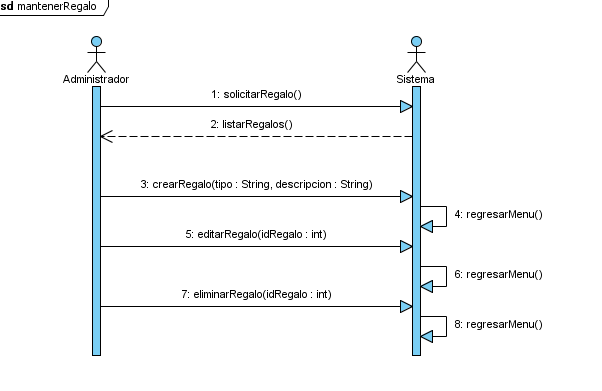
\includegraphics[height=10cm]{images/dss_mantenerRegalo.png}
% NO ME GUSTO EL UMBRELLO PARA HACER EL DIAGRAMA DX!
	% diagrama de secuencia del sistema que permita a un ejecutivo VIP asignar una entrada de un Evento a un cliente VIP
	\item DSS para Asignar una Entrada de un Evento a un Cliente VIP\\\\
		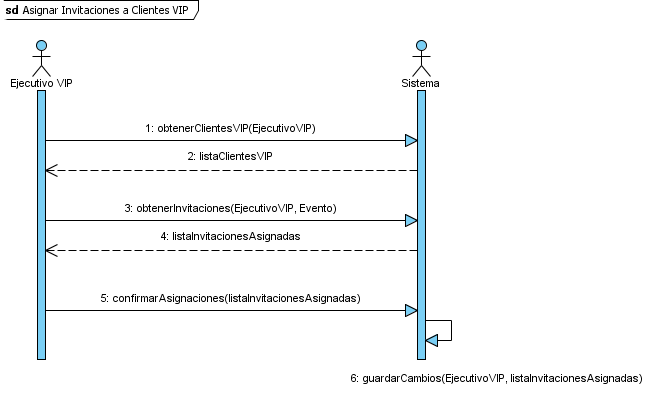
\includegraphics[height=10cm]{images/dss_invitacionesClienteVIP.png}

\end{enumerate}
% Yo le meti mano  y deberia estar listo.......... aunque esta muy chico :S!

\subsection{Contratos de las Operaciones Identificadas}
	\label{contratos_de_las_operaciones}
	
% contrato de las operaciones identificadas que tengan por post-condicion un cambio del estado del sistema (creacion/eliminacion/modificacion)

% NOTA: No es necesario poner las salidas, las referencias crusadas, notas y excepciones...
\begin{itemize}
	\item Contrato crearRegalo \\
	\begin{tabular}{|c|p{10cm}|}\hline
		Nombre: & crearRegalo\\\hline	
		Par\'ametros: & string tipo , string descripcion  \\\hline
		Responsabilidades: & Guardar en el sistema la definici\'on de un nuevo Regalo (su tipo y descripci\'on). \\\hline
		Tipo: & Sistema \\\hline
%		Referencias Cruzadas: &  \\\hline
%		Notas: &  \\\hline
		Excepciones: & Ya existe el regalo a ingresado \\\hline
%		Salidas: &  \\\hline
		Precondiciones: & El tipo de regalo debe ser \'unico. \\\hline
		Postcondiciones: &  Se crea una nueva instancia de Regalo, con idRegalo \'unico.\\\hline
	\end{tabular}
	\item Contrato editarRegalo \\
	\begin{tabular}{|c|p{10cm}|}\hline
		Nombre: & editarRegalo \\\hline	
		Par\'ametros: & int idRegalo \\\hline
		Responsabilidades: & Despliega los atributos del Regalo correspondiente (tipo y descripci\'on)
		para luego pasar a editar y guardar los cambios. \\\hline
		Tipo: & Sistema \\\hline
%		Referencias Cruzadas: &  \\\hline
%		Notas: &  \\\hline
		Excepciones: & El Regalo a editar no existe \\\hline
%		Salidas: &  \\\hline
		Precondiciones: & El idRegalo ingresado debe existir dentro de las instancias de Regalo.\\\hline
		Postcondiciones: & Se guardan los nuevos atributos en la instancia seleccionada. \\\hline
	\end{tabular}

	\item Contrato eliminarRegalo \\
	\begin{tabular}{|c|p{10cm}|}\hline
		Nombre: & eliminarRegalo\\\hline	
		Par\'ametros: & int idRegalo\\\hline
		Responsabilidades: & Elimina la instancia de Regalo que coincida con idRegalo \\\hline
		Tipo: & Sistena \\\hline
%		Referencias Cruzadas: &  \\\hline
%		Notas: &  \\\hline
		Excepciones: & El Regalo a eliminar no existe\\\hline
%		Salidas: &  \\\hline
		Precondiciones: & El idRegalo ingresado debe existir dentro de las instancias de Regalo. \\\hline
		Postcondiciones: & La instancia que coincida con idRegalo es eliminada. \\\hline
	\end{tabular}

%no modificaba nada >.<
%	\item ConfirmarAsignaciones\\
%	\begin{tabular}{|c|p{10cm}|}\hline
%		Nombre: & confirmarAsignaciones\\\hline	
%		Par\'ametros: & listaInvitacionesAsignadas \\\hline
%		Responsabilidades: & Validar que la sumatoria de las invitaciones asignadas a todos los Clientes VIP no supere la sumatoria de las Invitaciones asignadas al Ejecutivo VIP para el Evento\\\hline
%		Tipo: &  \\\hline
%%		Referencias Cruzadas: &  \\\hline
%%		Notas: &  \\\hline
%		Excepciones: &  \\\hline
%		Salidas: &  \\\hline
%		Precondiciones: & Ninguna \\\hline
%		Postcondiciones: &  \\\hline
%	\end{tabular}

	\item Contrato guardarCambios\\
	\begin{tabular}{|c|p{10cm}|}\hline
		Nombre: & guardarCambios\\\hline	
		Par\'ametros: & ejecutivoVIP, listaInvitacionesAsignadas \\\hline
		Responsabilidades: & Actualizar por cada Cliente VIP del ejecutivoVIP las invitaciones asignadas \\\hline
		Tipo: & Sistema \\\hline
%		Referencias Cruzadas: &  \\\hline
%		Notas: &  \\\hline
		Excepciones: & El ejecutivoVIP no tenia ninguna invitaci\'on asignada \\\hline
%		Salidas: &  \\\hline
		Precondiciones: & Se modificaron uno o m\'as de los valores editables de las invitaciones asignadas de los usuarios para el evento \\\hline
		Postcondiciones: & Se elimin\'o todas las invitaciones actualmente asignadas a los clientesVIP del ejecutivoVIP.\\ & Se crearon invitaciones y se asignaron para el clienteVIP y el Evento segun hallan sido ingresadas anteriormente y se establecieron los estados respectivos a cada invitaci\'on. \\\hline

	\end{tabular}

\end{itemize}

\subsection{Diagramas de Colaboracion de los Contratos}
	\label{diagramas_de_colaboracion}
	
% Por cada contrato que tengamos con postcondicion de cambio de estado hacer un Diagrama de Colaboracion en donde se expresen las decisiones de dise?o en torno a definir los mensajes que enviar y recibir.

	% Si uno considera que hay mas de 5, SOLO HACER 5, (los mas importantes segun su criterio).

\begin{itemize}
	\item crearRegalo\\\\
%		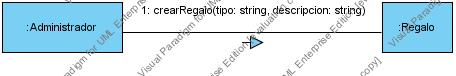
\includegraphics[height=10cm]{images/Diag_Colaboracion_crearRegalo.png}
		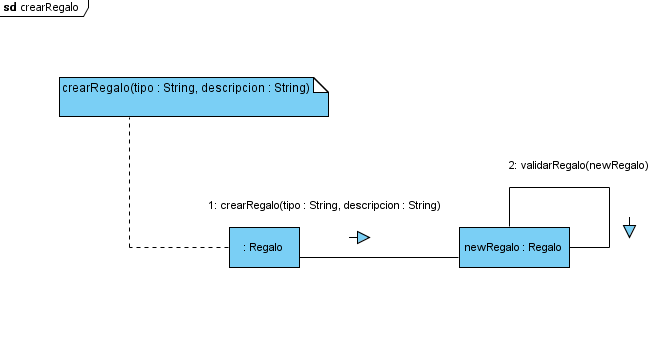
\includegraphics[width=16cm]{images/dc_crearRegalo.png}
	\item modificarRegalo\\\\
%		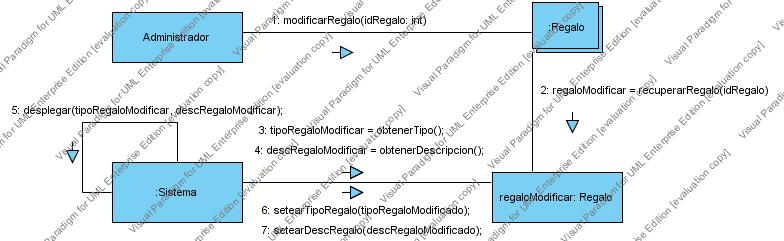
\includegraphics[height=10cm]{images/Diag_Colaboracion_modificarRegalo.png}
		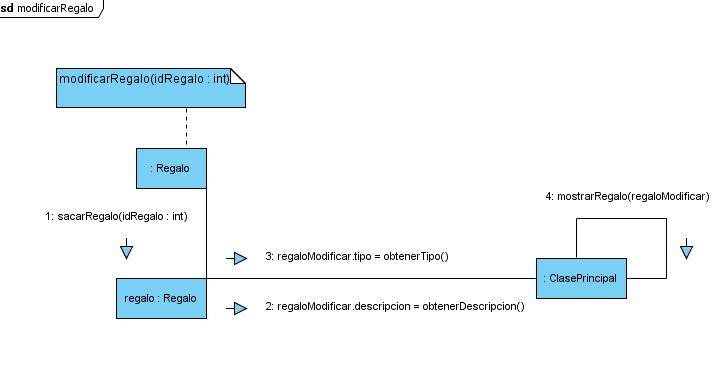
\includegraphics[height=9cm]{images/dc_modificarRegalo.png}
	\item eliminarRegalo\\\\
%		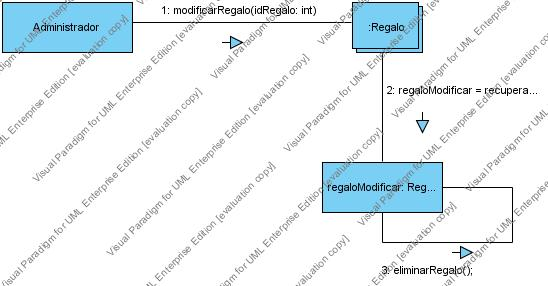
\includegraphics[height=10cm]{images/Diag_Colaboracion_eliminarRegalo.png}
		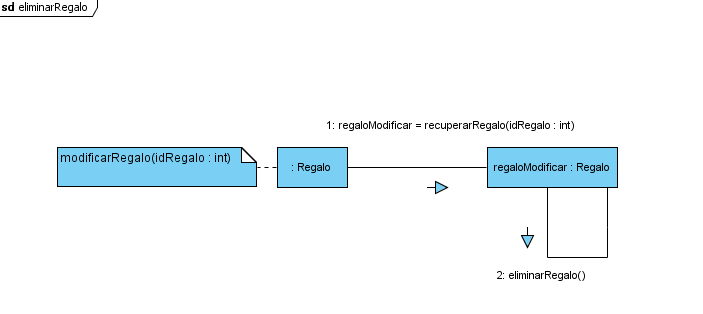
\includegraphics[width=16cm]{images/dc_eliminarRegalo.png}
%	\item Colaboracion 4
	\item guardarCambios\\\\
		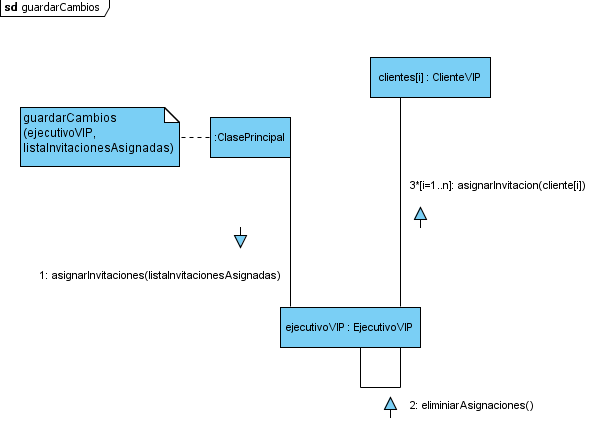
\includegraphics[height=10cm]{images/dc_guardarCambios.png}
\end{itemize}

\subsection{Diagramas de Clases}
	\label{diagramas_de_clases}
	
% Realizar los diagramas de clases consitentes con los diagramas de colaboracion

	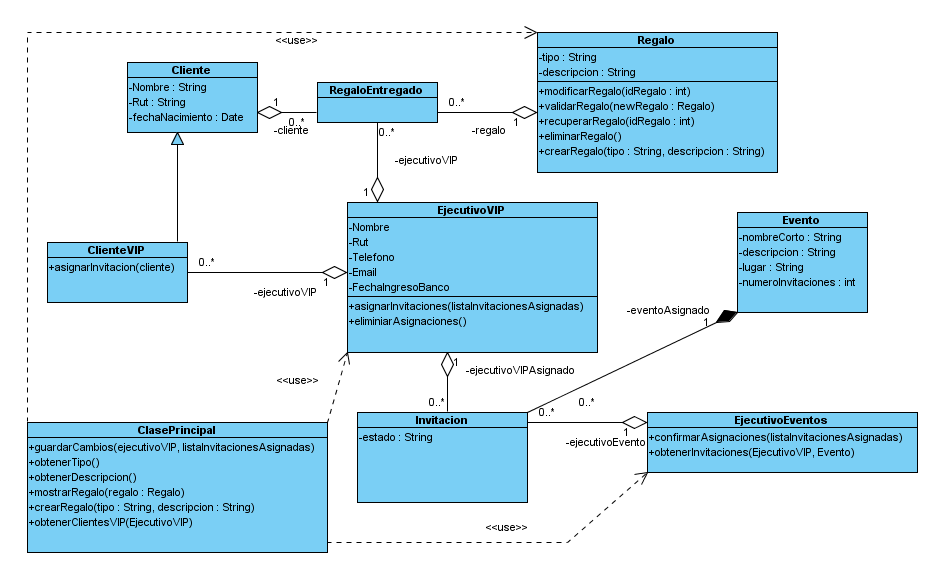
\includegraphics[height=11cm]{images/diagramaClases_tarea3.png}

\section{Supuestos Tarea 3}
	\label{sec:supuestos_t3}
	\begin{itemize}
	\item Las llamadas iniciales de los diagramas de comunicaci\'on fueron representadas como notas dado que no logramos representarlas como una llamada no numerada (y no logramos comenzar una llamada del vacio, el programa no lo permit\'ia).
	\item Se considero una clase 'clasePrincipal' que controla todas las operaciones del sistema general.
	\item Consideramos que seria bueno que el Administrador de Eventos sea identificable para poder reconocer a posterioridad que administrador de Eventos realizo los mejores eventos, o cometio errores al realizar algo.
	\item Se considero que el curso normal de los eventos, pueden haber diferentes Adminsitradores del Sistema trabajando paralelamente, por lo que habia que validar los datos para evitar inconsistencias en la base de datos.
	\item Se adaptaron  los diagramas seg\'un la pauta dada.
	\item Se considero que seg\'un el texto, el que manten\'ia los eventos era el Administrador de Eventos y no el Administrador del Sistema.
\end{itemize}


\section{Tarea 4}
\subsection{Prototipo de las pantallas del sistema (no funcional)}
	\label{prototipo_sistema}
	% colocar direccion al prototipo no funcional, navegable, del sistema

Se adjunta un directorio con todas las vistas de usuarios.\\
Desde el \emph{index.html} se pude navegar a todas las vistas(casos de uso), obviamente nada está funcional
ya que para eso deberia apoyarme en algun lenguaje dinámico como \emph{php}.\\
Siguiendo con lo mismo, no hay verificaciones, ni al momento de editar algo, que aparesca el valor anterior del campo.

\subsection{Diagramas de Clases considerando los patrones de dise\~no de alto nivel}
	\label{diagramas_de_clases_con_patrones}
	% Considerando los patrones de dise�o de alto nivel:

%       o Transfer Object (TO)
%       o Data Acces Object (DAO)
%       o Service Layer
%       o Model-View-Controller


%Realice un Diagrama de clases, donde identifique:
% -    Clases que controladoras de interfaz de usuario que deber�a construir, y
%     sus relaciones (usar estereotipo <<controller>) Hint: usar una por cada
%     p�gina HTML de su prototipo

% -    Clases que servir�n como Transfer Objects (usar estereotipo <<to>>) Hint:
%     considerar todos los Conceptos de Dominio sobrevivientes luego de los
%     refinamientos hechos durante los diagramas de colaboraci�n
%     Clases que tendr�n la responsabilidad de implementar los M�todos de

% -    Negocio,     y     sus      respectivos    m�todos    (usar    estereotipo
%     <<applicationService>>). Hint: use una sola clase para estos efectos.
%     Incorpore todos los m�todos que realizan validaciones y cambios de estado
%     persistentes en el sistema.

% -    Clases que tendr�n la responsabilidad de implementar los m�todos de
%     acceso a datos, requeridos por los M�todos de Negocio, y sus respectivos
%     m�todos (usar estereotipo <<dao>>). Hint: use una sola clase para estos
%     efectos. Incorpore todos los m�todos que realizan obtenci�n de datos,
%     actualizaci�n y creaci�n de datos en la base de datos

% Utilice un diagrama por cada uno de los patrones.


\section{Supuestos Tarea 4}
	\label{sec:supuestos_t4}
	\begin{itemize}
	\item Se considero una clase 'clasePrincipal' que controla todas las operaciones del sistema general.
	\item Consideramos que seria bueno que el Administrador de Eventos sea identificable para poder reconocer a posterioridad que administrador de Eventos realizo los mejores eventos, o cometio errores al realizar algo.
	\item Se considero que el curso normal de los eventos, pueden haber diferentes Adminsitradores del Sistema trabajando paralelamente, por lo que habia que validar los datos para evitar inconsistencias en la base de datos.
	\item Se adapt\'o el diagrama de casos de uso segun la pauta dada en la tarea.
	\item Se considero que seg\'un el texto, el que manten\'ia los eventos era el Administrador de Eventos y no el Administrador del Sistema.
\end{itemize}


%\section{Descripci\'on herramienta utilizada: Umbrello}
%	\label{sec:umbrello}
%	\begin{center}
	
\includegraphics[height=1.5cm]{images/umbrello}\\
\end{center}
\textbf{Umbrello} es una herramienta libre para crear y editar diagramas UML, que ayuda en el proceso del desarrollo de software. Fue desarrollada por Paul Hensgen, y está diseñado principalmente para KDE, aunque funciona en otros entornos de escritorio.\\

Umbrello maneja gran parte de los diagramas estándar UML pudiendo crearlos, además de manualmente, importándolos a partir de código en C++, Java, Python, IDL, Pascal/Delphi, Ada, o también Perl (haciendo uso de una aplicación externa). Así mismo, permite crear un diagrama y generar el código automáticamente en los lenguajes antes citados, entre otros. El formato de fichero que utiliza está basado en XMI.\\

También permite la distribución de los modelos exportándolos en los formatos DocBook y XHTML, lo que facilita los proyectos colaborativos donde los desarrolladores no tienen acceso directo a Umbrello o donde los modelos van a ser publicados vía web.Umbrello se distribuye en el módulo kdesdk de KDE.\\

\textbf{Web:} http://uml.sourceforge.net/


\end{document}
